\chapter{\IfLanguageName{dutch}{Stand van zaken}{State of the art}}%
\label{ch:stand-van-zaken}

% Tip: Begin elk hoofdstuk met een paragraaf inleiding die beschrijft hoe
% dit hoofdstuk past binnen het geheel van de bachelorproef. Geef in het
% bijzonder aan wat de link is met het vorige en volgende hoofdstuk.

% Pas na deze inleidende paragraaf komt de eerste sectie hoofding.

%Dit hoofdstuk bevat je literatuurstudie. De inhoud gaat verder op de inleiding, maar zal het onderwerp van de bachelorproef *diepgaand* uitspitten. De bedoeling is dat de lezer na lezing van dit hoofdstuk helemaal op de hoogte is van de huidige stand van zaken (state-of-the-art) in het onderzoeksdomein. Iemand die niet vertrouwd is met het onderwerp, weet nu voldoende om de rest van het verhaal te kunnen volgen, zonder dat die er nog andere informatie moet over opzoeken \autocite{Pollefliet2011}.

%Je verwijst bij elke bewering die je doet, vakterm die je introduceert, enz.\ naar je bronnen. In \LaTeX{} kan dat met het commando \texttt{$\backslash${textcite\{\}}} of \texttt{$\backslash${autocite\{\}}}. Als argument van het commando geef je de ``sleutel'' van een ``record'' in een bibliografische databank in het Bib\LaTeX{}-formaat (een tekstbestand). Als je expliciet naar de auteur verwijst in de zin, gebruik je \texttt{$\backslash${}textcite\{\}}.
%Soms wil je de auteur niet expliciet vernoemen, dan gebruik je \texttt{$\backslash${}autocite\{\}}. In de volgende paragraaf een voorbeeld van elk.

%\textcite{Knuth1998} schreef een van de standaardwerken over sorteer- en zoekalgoritmen. Experten zijn het erover eens dat cloud computing een interessante opportuniteit vormen, zowel voor gebruikers als voor dienstverleners op vlak van informatietechnologie~\autocite{Creeger2009}.

%\lipsum[7-20]

Het doel van dit onderzoek is meer inzicht te verschaffen in het gebruik van containertechnologie, toegepast op installatie van Hadoop, Spark en Kafka, om de software die nodig is voor het vak Big Data Processing aan HOGENT zoveel mogelijk te automatiseren.
\newline
Meer concreet worden tijdens deze oefeningen de applicaties Hadoop, Spark en Kafka geïnstalleerd tijdens de les. Lestijd die beter kan besteed worden aan bijvoorbeeld het gebruik van de applicaties.
\newline
\newline
Een extra doelstelling is om met het resultaat van deze studie deze applicaties ook tijdens de examens te kunnen gebruiken op een centrale installatie van HOGENT, met inachtname van veiligheid en stabiliteit.
\newline
\newline
Gezien het doel van deze studie is om te komen tot inzichten en aanbevelingen voor een installatie ter ondersteuning van de oefeningen, in de eerste instantie, zal het onderzoek rekening houden met de functionaliteiten die tijdens de les gebruikt worden. We stippen aan dat we hierbij niet ingaan op de volledige werking van de applicaties.
\newline
\newline

\section{Container technologie}
Een container biedt een omgeving waarbinnen één of meerdere applicaties draaien. Container technologie gebruikt de TODO virtualisatie mogelijkheden van het Operating Systeem om meerdere containers geïsoleerd van elkaar te draaien binnen 1 machine. Daarbij wordt de kernel van het Operating Systeem van de machine gedeeld door alle containers.
\newline
Dit is in tegenstelling tot virtuele machines, waar telkens een volledige `virtuele computer` wordt gebruikt, inclusief het Operating Systeem. Hierdoor zijn containers veel kleiner, zowel wat disk space als geheugen betreft.
\newline
Merk op dat de machine waarbinnen de containers draaien zowel een fysieke als een virtuele machine kan zijn.
\newline
Twee typische voorbeelden van container technologie zijn LXC (LinuX Containers) en Docker. TODO Referentie
\newline
LXC draait enkel op Linux en biedt een container die in essentie een blanco Linux omgeving is, waarbinnen dan 1 of meerdere applicaties worden geïnstalleerd. Als Linux omgeving is er zeer veel flexibiliteit maar daaraan gekoppeld ook meer complexiteit.
\newline
Docker heeft aan containers een aantal functionaliteiten toegevoegd zoals abstractie van opslag en netwerk, en het concept van 'image' dat beter is ondersteund en effiënter qua disk space. Een image bevat al het nodige om een applicatie te kunnen draaien (code, ondersteunende software bijvoorbeeld Java Virtual Machine, scripts, configuratie), dit laat toe om een Docker container eenvoudig op te zetten gebaseerd op voorgedefinieerde images.
\newline
Een essentieel verschil met LXC containers is dat Docker containers 'single-process' zijn. Dit betekent dat ze 1 enkel proces draaien. Vandaar ook de typische aanpak van Docker images waarbij elk image 1 enkele applicatie bevat, inclusief de ondersteunende software en de bijhorende configuratie. Dat maakt dat een Docker image telkens gelinkt is aan 1 oplossing.
\newline
\begin{figure}[H]
    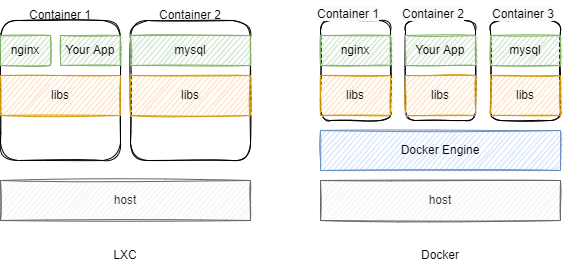
\includegraphics[scale=0.8]{LXC vs Docker.png}
    \caption{Het verschil tussen LXC en Docker containers \autocite{Kahuha2023}.}
\end{figure}

Uitgevers van software, zowel Open Source als commerciële software, stellen dikwijls hun oplossing ook ter beschikking op DockerHub als image, en aangezien iedereen toegang kan krijgen tot DockerHub, binnen bepaalde limieten afhankelijk van het gratis of betalende abonnement, worden Open Source images ook door derden toegevoegd.
\newline
Voor developers is het voordeel dat ze snel een lokale omgeving kunnen opstaren, van een bepaalde versie van een oplossing, bijvoorbeeld MySQL, nginx, enz. Voor het ene project is MySQL versie 5.x nodig, voor een ander project MySQL 8.x, hiervoor moet de development omgeving niet telkens gewijzigd worden, per project wordt de ondersteunende software via containers gestart.
\newline
Als onderdeel van een CI/CD pipeline worden images gebouwd en daarna van Test naar Acceptatie naar Productie omgeving gebracht, hetzelfde ongewijzigde image dus minder kans op fouten tijdens installatie. Bij containers gebeurt de bouw van de image geautomatiseerd 1 keer. Daarna is het de image die alle omgevingen doorloopt.
\newline
In grootschalige cloud-omgevingen is het voordeel van image gebaseerde containers dat bijkomende containers opstarten veel eenvoudiger is. Hiervoor zijn intussen ook al oplossingen gegroeid zoals Kubernets zie verder.
\newline
In de eerste versies maakte Docker gebruik van LXC, voor de virtualisatie functionaliteiten, maar in recentere versies is er een eigen onderliggende technologie gebouwd als virtualisatie laag, die vooral kon steunen op het concept dat er maar 1 applicatie per container draait. 
\newline
\newline

Voor een nog meer gedetailleerde vergelijking verwijzen we naar \textcite{Tunggal2023}.

\subsubsection{Docker Image opbouw en structuur}
Docker images gebruiken een `parent` image, bijvoorbeeld een basis Linux container image, waaraan dan op basis van de Dockerfile (een tekst file met opeenvolgende commandos) software wordt toegevoegd. De nieuwe image verwijst naar de parent image, maar bevat deze niet. Er wordt een `laag` aangemaakt die dan samen met de parent image kan uitgevoerd worden. Samen vormen ze de nieuwe image.
Deze kan op zijn beurt gebruikt worden als parent voor een andere image, die dan al uit 3 image lagen zal bestaan. Dit vormt een besparing op disk space en netwerk communicatie, want de images worden typisch centraal opgeslagen op DockerHub zodat ze door anderen kunnen gebruikt worden.
Merk op dat dit betekent dat de inhoud van deze image layers niet kan gewijzigd worden, anders zou de container met Image A gebaseerd op Image X de inhoud wijzigen van Image B ook gebaseerd op Image X. 

\subsection{Volume}
Om de container toe te laten gegevens te bewaren introduceert Docker het concept van een volume. Dit is een opslagplaats waarvan de container kan gebruikmaken. Volgens  \textcite{Frieze2022} zijn er tijdelijke volumes die terug worden verwijderd eens de container stopt, en volumes die worden gecreëerd buiten de container, en dus deel uitmaken van de Docker omgeving waar de container draait, en blijven bestaan buiten de levensduur van de container.
\newline
Bijvoorbeeld voor een database container worden de databases zelf in een vast volume bewaard anders zou alles verloren gaan eens de container stopt.

\subsection{Docker-compose}
Volgens \textcite{Docker2023} is Docker Compose een onderdeel van de Docker software dat helpt om combinaties van Docker containers samen te gebruiken. De basis vormt een Docker Compose file (yaml formaat) waarin verschillende containers (services genaamd in Docker Compose terminologie) worden gedefinieerd. Elke service is gebaseerd op een Docker image, per service kunnen er volumes toegevoegd worden, netwerken opgezet die toelaten aan de verschillende containers om te communiceren, dependencies tussen services (welke eerst moet gestart worden), parameters die bepalen wanneer een container moet herstart worden, enz.
\newline
\newline
De meeste van die zaken zijn allemaal ook manueel te verwezenlijken met meerdere opeenvolgende Docker commando's maar het voordeel van Docker Compose is dat het toelaat dit op een declaratieve manier vast te leggen in één file en met één enkel docker compose commando wordt de combinatie van services opgestart. De Docker compose file kan ook makkelijk gedeeld en herbruikt worden, met beperkte aanpassingen versies wijzigen, het geheel van de container samenhang zit in \'e\'en file.
\newline
\newline

\subsection{Container technologie conclusie}
Als containertechnologie is Docker gekozen voor de volgende redenen:
\newline
\begin{itemize}
    \item Het is vandaag de meest gebruikte container TODO (bewijs) technologie en wordt ondersteund door grote bedrijven zoals Red Hat, Canonical, Oracle, Microsoft en Google. Exacte en onafhankelijke cijfers die de populariteit van containertechnologie vergelijken zijn niet gevonden, maar het is wel tekenend dat bij herhaaldeljk zoeken naar container technologie je altijd resultaten krijgt voorgesteld die over Docker gaan.
    \item De VIC omgeving: Docker en Docker Compose worden vandaag al gebruikt in het VIC (zie verder).
    \item De 3 Big Data applicaties zijn ieder apart beschikbaar als Docker container image en moeten dus niet meer zelf gebouwd of geïnstalleerd worden. Met de images kunnen TODO we direct aan de slag om combinaties op te zetten, en via configuratie aan te passen aan de vereisten.
    \item Hadoop heeft YARN als resource manager (zie verder) en deze kan Docker gebruiken om zelf containers te starten. In dit geval draaien er bijvoorbeeld meerdere machines een Hadoop nodemanager en kan YARN op elk van deze machines meerdere containers opstarten. YARN en Hadoop worden verder nog besproken \autocite{Hadoop2023a}.
\end{itemize}

De voorgestelde oplossing zou kunnen bestaan uit meerdere docker-compose files, telkens voor één van de Big Data applicaties of een combinatie ervan. Zoals ook verder beschreven bestaat elke applicatie uit meerdere processen die elk in één container kunnen draaien. Dit zullen we verder moeten uitzoeken.
\newline
\newline

\subsection{Docker en containerd}
Om het voorgaande enigzins overzichtelijk te houden, en ook om historische redenen want ``docker'' was de eerste tool van Docker, spraken we over ``Docker'' containers als overkoepelende benaming van alle functionaliteit die geboden wordt maar er zit intussen veel meer achter dan enkel de docker tool, die nu is hernoemd naar Docker Desktop (voor Developers op Windows, Mac en Linux) en Docker Engine (voor servers op Linux).
De Docker Engine bestaat uit de Docker daemon, die draait in de achtergrond en containers beheert, en de docker-cli tool, die toelaat om via command-line instructies te geven aan de Docker Daemon.
De Docker Daemon gebruikt zelf dan weer ``containerd'', een daemon en container runtime die gestandardiseerd en onafhankelijk (afgesplitst) is van Docker. Het zou ons te ver leiden om hier dieper op in te gaan maar 2 punten zijn van belang om te onthouden:
\begin{itemize}
    \item containerd ondersteunt de Docker images en kan deze uitvoeren. Het is dus mogelijk de Docker images te gebruiken in oplossingen die de Docker container niet of niet langer onderliggend gebruiken maar vervangen hebben door de meer standaard containerd
    \item Kubernetes (zie verder) is zo'n oplossing die initieel beroep deed op Docker maar intussen containerd rechtstreeks gebruikt.
\end{itemize}

Een goede introductie tot dit alles is te vinden in \textcite{Donohue2023}.


\subsection{Cluster}
Een cluster is een groep van computers, clusternodes genaamd, die samenwerken en zich naar de gebruiker toe als 1 enkel systeem gedragen. Het concept van een cluster is dat het werk wordt verdeeld over de verschillende nodes.
Dit heeft meerdere voordelen:
\newline
\begin{itemize}
    \item Door de architectuur van samenwerking kan een cluster eenvoudig en in theorie ongelimiteerd uitgebreid worden met bijkomende nodes, in tegenstelling tot oplossingen die slechts op 1 enkele machine draaien en die dan beperkt worden door de fysieke limieten van de machine (Scalability).
    \item Bij de meeste applicaties is de belasting niet continu dezelfde en een cluster architectuur laat toe om, volgens de actuele vraag, bijkomende nodes op te starten en later terug af te sluiten. Dit spaart resources en maakt nodes ook beschikbaar voor andere applicaties.
    \item Instabiele nodes kunnen worden herstart zonder dat de gebruiker er iets van merkt (Stability; Availability).
\end{itemize}

\subsection{Docker Swarm}
Volgens \textcite{Docker2023b} worden bij een Docker cluster, ook Docker Swarm genoemd, de containers verdeeld over verschillende nodes door cluster management van de Docker engine zelf. Een swarm bestaat uit meerdere Docker hosts, waarop zowel een manager als een worker kunnen draaien, en waarbij de managers de gewenste containers verdelen over de worker nodes, rekening houdende met specificaties zoals welke opslag resources, netwerken en aantal instanties gewenst zijn. De Docker engine zorgt voor de connectiviteit tussen de containers.
\newline
\newline
Docker Swarm is dus een mogelijkheid voor de installatie en het beheer van Big Data oplossingen.
\newline
\newline

\subsection{Kubernetes}
Kubernetes, of K8s, is een open-source container oplossing ontworpen door Google. Het wordt gebruikt om groepen of clusters van applicaties binnen containers te beheren. Dit noemen we in de IT wereld ‘orkestratie’.
\newline
Kubernetes start en monitort containers, start extra containers indien nodig om de belasting aan te kunnen, en stopt en herstart automatisch containers die niet langer reageren \autocite{Guthrie2022}.
\newline
\newline
De laatste jaren worden containers meer en meer gebruikt en Kubernetes is zowat de standaard geworden voor bedrijven om hun containers te beheren en te automatiseren \autocite{Razorops2022}.
\newline
\newline
Een belangrijk onderdeel van Kubernetes is de netwerk communicatie. Er zijn meerdere types communicatie, namelijk die tussen containers in eenzelfde pod (eenvoudig gebruik van localhost), die tussen pods onderling, en die van de buitenwereld naar een service, deze laatste is een manier om toegang te verlenen tot een applicatie die binnen de cluster op meerdere pods draait \autocite{Kubernetes2023a} \autocite{Kubernetes2023b}.
\newline
\newline
Kubernetes is ook een mogelijke oplossing voor de automatisatie van installatie van de Big Data oplossingen.


\subsection{Docker Swarm en Kubernetes}
Docker Swarm en Kubernetes bieden vergelijkbare functionaliteiten voor het beheer van de levenscyclus van containers.

Zowel \textcite{Rosen2022} als \textcite{Chukwudi2023} vinden dat Kubernetes meer gebruikt wordt en een grotere community heeft. Het is krachtiger maar daarmee komt ook complexiteit en het feit dat het veel moeilijker is om te leren gebruiken.
Beiden vinden Docker Swarm veel eenvoudiger in gebruik en geschikter voor kleinere omgevingen. Het gebruikt ook minder resources dan Kubernetes.
\newline
Toegepast op HOGENT en het VIC lijkt Docker Swarm dus de betere keuze.


\section{Hadoop}
De eerste Big Data oplossing die werd bekeken is Apache Hadoop. Dit is een raamwerk dat toelaat om grote sets van gegevens gedistribueerd te verwerken, waarbij die verdeling over clusters van computers toegankelijk is via eenvoudige programmeermodellen en de gegevens worden opgeslagen in het gedistribueerde filesysteem HDFS.
\newline
Hadoop is ontworpen om als cluster gebruikt te worden, met fout detectie en afhandeling ervan, en kan gaan tot duizenden machines, elk met lokale verwerking en opslag. \autocite{ASF2022}

\subsection{Hadoop Distributed File System}
Om de data te verdelen over alle nodes die deelnemen aan de Hadoop cluster wordt het Hadoop Distributed File System of HDFS gebruikt, dit heeft een \newline master/slave architectuur en laat toe om gegevens op te slaan in files die verdeeld worden over de cluster. Een cluster bestaat uit 1 master, de namenode en meerdere slaves, de datanodes. Een 2de namenode kan worden gebruikt als backup om de stabiliteit van de cluster te verzekeren.
\newline
De namenode houdt bij in welke datanodes de data zich bevinden. Meerdere kopieën van de data worden gerepliceerd over de verschillende datanodes zodat er geen data verloren gaat bij uitvallen van een datanode.
\newline
\newline
Initieel was HDFS bedoeld om een goede performantie en stabiliteit te garanderen op eerder goedkope hardware, en om het mogelijke falen hiervan op te vangen werd het ontworpen met een focus op verdeling en redundantie van de data. De ``fault-tolerance'' wordt op die manier verzekerd door de software en niet door high-end hardware.
Door de architectuur van HDFS biedt het een goede performantie voor applicaties die nood hebben aan het verwerken van zeer grote datasets \autocite{Borthakur2007}.
\newline
\newline
\subsection{MapReduce}
MapReduce is een programmeermodel en framework dat deel uitmaakt van Hadoop. Het doet beroep op de kracht van het Hadoop Distributed File System om de data die verwerkt moet worden te verdelen over grote aantallen nodes en daar parallel te verwerken \autocite{Talend2023}.

Kort uitgelegd is MapReduce gebaseerd op 2 functionaliteiten: \textbf{map} en \textbf{reduce}.
\newline
\newline
De Data die verwerkt moet worden, doorloopt de volgende fases die telkens in parallel worden uitgevoerd:
\begin{itemize}
    \item \textbf{Opsplitsing}: grote volumes data worden opgesplitst en verdeeld over de HDFS nodes.
    \item \textbf{Map}: elk deeltje data wordt bewerkt met de map functie en omgezet in sleutel-waarde paren (key-value pairs).
    \item \textbf{Herschikken en Sorteren}: De data-paren worden hergroepeerd op basis van de sleutels.
    \item \textbf{Reduce}: de reduce functie ontvangt de herschikte data en zal die aggregeren (= reduceren) en het resultaat terug aan HDFS geven.
\end{itemize}

De volgende figuur verduidelijkt de werking van MapReduce met een voorbeeld van verwerken van tekst, waarbij de woordfrequentie wordt berekend door de data eerst te splitsen en uiteindelijk terug samen te voegen. In de fases van Mapping en Reducing wordt  het werk uitgevoerd door meerdere onafhankelijke processen.
\begin{figure}[H]
    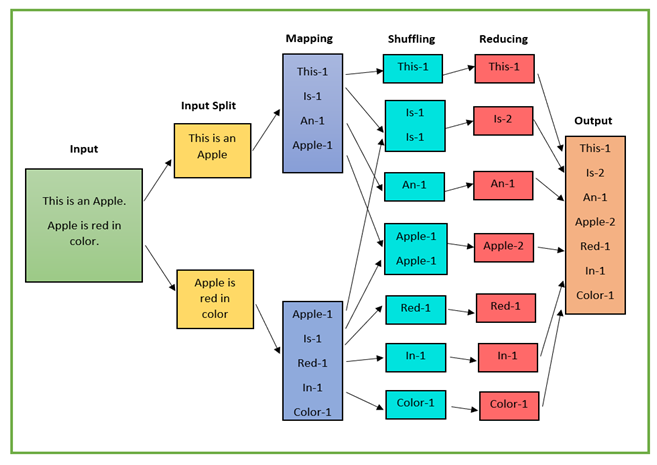
\includegraphics[scale=0.9]{map-reduce.png}
    \caption{Diagram ter verduidelijking van MapReduce \autocite{Anushkakhatri2022}.}
\end{figure}

Hadoop ondersteunt het gebruik van MapReduce programmas geschreven in programmeertalen zoals Java, Python, Ruby en C++ 
\autocite{Taylor2023}.
\newline
\newline
Hadoop wordt o.a. alleenstaand gebruikt tijdens de oefeningen Big Data Processing, daarvoor kunnen we bestaande Docker Compose files gebruiken die de verschillende services bevatten nodig om een Master of Slave te starten.
In de eenvoudigste vorm is er \'e\'en docker compose file die alle services opstart om te kunnen werken met \'e\'en master en \'e\'en slave.
\newline
\newline
Elke service (namenode, datanode, resourcemanager) is een specifiek Docker image, waarvan er voorbeelden te vinden zijn op DockerHub, en ook van de Docker scripts die gebruikt werden om de images op te bouwen. Typisch is er een basis Hadoop image dat het volledige framework bevat, en worden daar aparte images vanaf geleid die telkens maar 1 specifiek process (namenode, datanode, ...) van Hadoop opstarten.
\newline
Door op die manier met aparte images te werken kan het beheer van de cluster buiten Hadoop worden gedaan, bijvoorbeeld in Kubernetes of Docker Swarm.
\newline
\newline
In de volgende sectie gaan TODO we Apache Spark bekijken, welke functionaliteit dit toevoegt aan Hadoop en hoe TODO we dit kunnen integreren.
\newline
\newline

\section{Spark}
Apache Spark is net als Hadoop een Open Source framework bedoeld voor het verwerken van grote datasets. Volgens \textcite{AwsAmazon2023a} verdeelt Spark ook de gegevens en de taken over verschillende nodes, maar houdt het data daarbij zoveel mogelijk in cache (RAM geheugen), in plaats van in een bestandssysteem. Voor bepaalde gevallen zal het dus veel sneller zijn dan Hadoop.
\newline
\newline
De data in Spark wordt verdeeld opgeslagen in de cluster, in eerdere versies in RDD (Resilient Distributed Dataset), een set van data objecten in Java of Scala formaat. In nieuwere versies van Spark wordt DataFrame gebruikt, waarbij de gegevens gestructureerd worden in kolommen, gelijkaardig aan een tabel in een relationele databank. Volgende componenten zijn aanwezig in Spark om dit soort gestructureerde data te helpen verwerken: Spark SQL, Spark MLlib en Spark GraphX.
\autocite{DataFlair2023}
\newline
\newline

\subsection{Spark SQL, DataFrames and Datasets}
Deze module is de meest gebruikte Spark module voor gestructureerde data verwerking en laat toe om data op te halen en te bewerken door middel van SQL APIs, DataFrame APIs en Dataset APIs, waarvoor bibliotheken beschikbaar zijn voor meerdere programmeertalen waaronder Java, Scala en Python. Voor deze laatste bestaan alleen de eerste 2 APIs, niet de Dataset APIs.
De API voelt vertrouwd aan en begint met het openen van een Spark sessie via dewelke de data dan kan opgehaald worden uit een hele resem ondersteunde data sources (json, csv, text, hive, avro). Het ophalen gebeurt door gebruik te maken van de APIs, aangevuld met SQL instructies voor filteren en sorteren, waarna de data als Dataframe dan verder kan verwerkt worden.
De SQL interface kan ook aangesproken worden via jdbc en odbc.
(Volgens \textcite{Spark2023}, \textcite{Naveen2023}, \textcite{Spark2023a})

\subsection{Spark MLlib}
De Machine Learning Library (MLlib) van Apache Spark is ontworpen voor eenvoud en schaalbaarheid  en bestaat uit leeralgoritmen en hulpprogramma's, waaronder classificatie, regressie, clustering, collaboratieve filtering en onderliggende optimalisatie. Spark MLLib ondersteunt het trainen van modellen en daarop gebaseerde data voorspellingen, en integreert met de andere Spark-componenten. Het is beschikbaar voor meerdere programmeertalen waaronder Java, Scala en Python.
Spark MLlib biedt zowel een Dataframe API als eerste keus als een RDD API die intussen lijkt uitgefaseerd te worden.
(Volgens \autocite{Spark2023b})

\subsection{Spark GraphX}
Spark GraphX is een Spark API die toelaat om grafen op te bouwen, gebaseerd op achterliggende databronnen in Spark, en hierop dan parallelle verwerking en analyses te doen. 
Een graaf is een data structuur die bestaat uit een verzameling objecten, knopen, en hun onderliggende relaties, verbindingen. Dit kun je duidelijk zien op figuur 2.3.
\newline
\newline
\begin{figure}[H]
    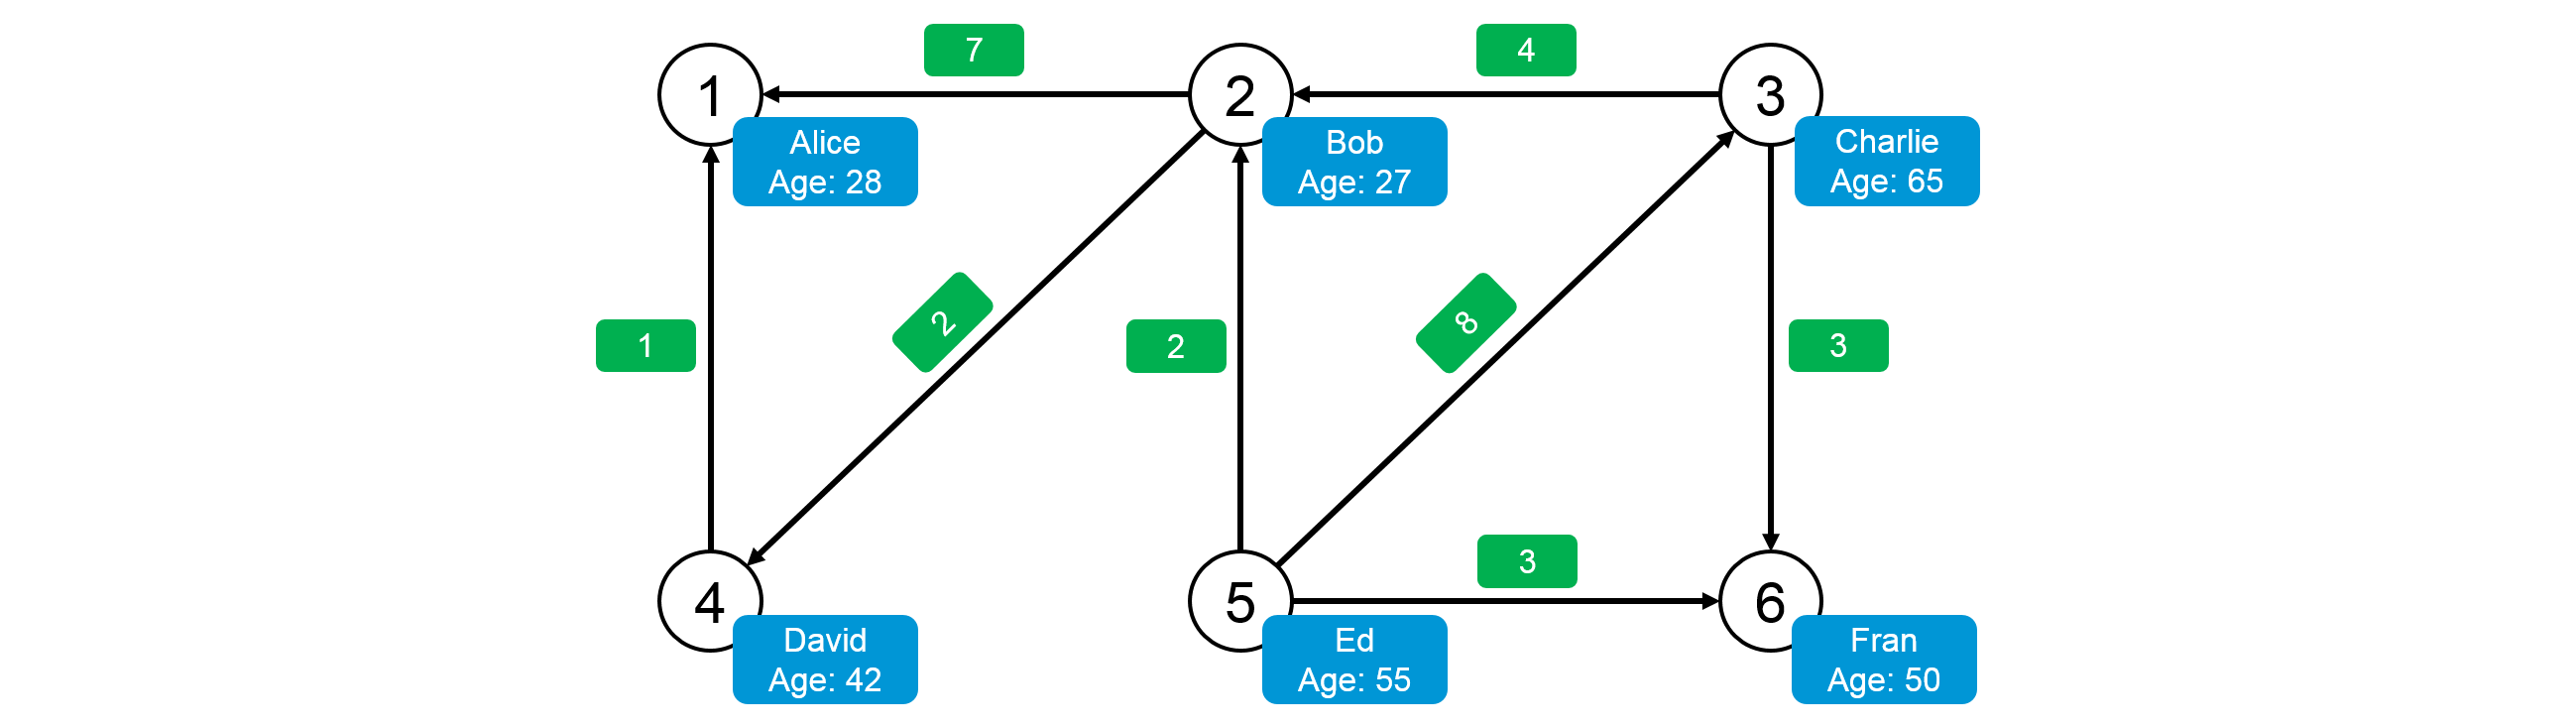
\includegraphics[scale=0.2]{GraphX-Example-Spark-GraphX-Tutorial-Edureka.png}
    \caption{Voorbeeld van een graaf \autocite{Dayananda2019}.}
\end{figure}


\subsection{Spark Streaming / Structured Streaming}
Volgens \autocite{Buuck2022} is Spark Streaming een uitbreiding van de Spark APIs, die toelaat de verwerking te doen van ``Live'' data, data streams genaamd. Intussen wordt het als legacy beschouwd en is het vervangen door ``Structured Streaming'' dat gelijkaardige functionaliteit biedt door gebruik te maken van de DataFrame APIs in plaats van de Streaming RDD APIs. Met als voordeel dat SQL beter ondersteund wordt in de DataFrame APIs.
\newline
\newline
Het is dit laatste onderdeel van Spark, Structured Streaming, dat typisch in combinatie met Kafka (zie verder) wordt gebruikt om data op te halen en na verwerking terug te bezorgen voor eventuele verdere stappen.
\newline
\newline
Terugkomend op ons doel van Spark in containers te draaien: er zijn Spark Docker images beschikbaar die toelaten zowel een Spark Master als een Spark Worker te starten.


\section{Kafka}
Volgens \textcite{AwsAmazon2023b} is Apache Kafka een Open Source gedistribueerd platform voor Event Streaming, waarbij binnenkomende boodschappen (events) continu worden opgeslagen en verwerkt. Het wordt gebruikt voor data-pijplijnen en data-integratie applicaties.
Volgens \textcite{ASF2022b} is het schaalbaar tot duizenden Brokers, kan het billioenen boodschappen per dag aan en is het zeer fault-tolerant door de cluster-architectuur. Hieronder worden een aantal typische concepten van Apache Kafka besproken.

\subsection{Kafka Broker}
Volgens \textcite{GitBook2023} bestaat een Kafka cluster uit meerdere servers, en deze servers worden brokers genoemd. Brokers binnen een cluster praten rechtstreeks met elkaar en via Zookeeper (zie verder).
\newline
De belangrijkste taak van een broker is het ontvangen en opslaan van Records.

\subsection{Een Event of Kafka record}
Een event is een boodschap die doorgeeft dat er ``iets'' is gebeurd, van belang voor de applicatie die wordt gebouwd. Deze boodschap bevat informatie over datgene dat is gebeurd en bevat een tijdstip, een sleutel, specifieke waardes en eventuele bijkomende metadata. Een voorbeeld uit de bankwereld van zo'n event is ``Piet Peeters'' ``heeft een betaling van 123Euro gedaan aan Jan Janssens'' op ``10/02/2023 om 11:35''.
\newline
In de terminologie van Kafka worden events gestuurd door ``Producers'' naar Kafka, waar ze worden opgeslagen en daarna kunnen worden opgevraagd door ``Consumers''. Doordat beiden enkel via Kafka communiceren zijn ze van elkaar losgekoppeld en is dus de producer niet afhankelijk van de beschikbaarheid van de consumer \autocite{Kafka2023}.
\newline
Daarnaast kunnen eenvoudig meerdere consumers bijgekoppeld worden zonder dat de producer hiervan op de hoogte hoeft te zijn of worden aangepast.
\newline
Dit wordt ook wel het ``Publish-Subscribe'' mechanisme genoemd. Er is 1 partij die events publisht en er zijn 1 of meerdere partijen die subscriben op de events van de Publisher.
In de terminologie van Kafka vormt een event een record dat opgeslagen wordt.


\subsection{Kafka Topic}
Volgens \textcite{Harbour2023} kan een topic gezien worden als een soort logisch kanaal waarlangs de communicatie tussen producer en consumer verloopt. Een producer stuurt dus Events naar een specifiek topic en een consumer gaat Events opvragen in datzelfde topic. Het topic is dus een begrip dat beiden kennen en een manier om ze aan elkaar te koppelen.


\subsection{Kafka Partition}
Een topic bestaat uit 1 of meerdere partities. Records worden in een partitie opgeslagen door ze telkens achteraan de partitie toe te voegen. Bij het lezen van een topic/partitie ontvangen de consumers de records in dezelfde volgorde als ze gestuurd werden door de producer, dit is telkens enkel geldig bij één enkele topic/partitie. De volgorde van records die niet in eenzelfde partitie zijn opgeslagen is onbepaald.
Meerdere partities voor 1 enkel topic dienen ter ondersteuning van de schaalbaarheid, waarbij elke partitie wordt opgeslagen op een andere broker. Op die manier kunnen topics met zeer grote volumes aan records parallel opgeslagen en verwerkt worden.
\newline
\newline
Volgens \textcite{Harbour2023} speelt de sleutel van een event een belangrijke rol bij partitions. Voor het verwerken van grote volumes aan events kunnen meerdere consumers opgezet worden die ieder de events van een enkele partitie verwerken. Die consumers krijgen de events van hun partitie in de juiste volgorde binnen, maar zien niet de events op de andere partities. Terugkerend naar ons voorbeeld uit de bankwereld:
\begin{itemize}
    \item Producer stuurt een event dat 100 Euro op de rekening van Jan wordt gezet. Dit wordt op partitie 1 gezet.
    \item Producer stuurt een event dat 50 Euro van de rekening van Jan wordt gehaald. Dit wordt op partitie 2 gezet.
    \item Consumer X leest van de partitie 2 dat 50 Euro van de rekening van Jan wordt gehaald -> dit wordt geweigerd want er staat niet genoeg geld op.
    \item Consumer Y leest van de partitie 1 dat 100 Euro op de rekening van Jan wordt gezet -> dit wordt uitgevoerd.
\end{itemize}

\begin{figure}[H]
    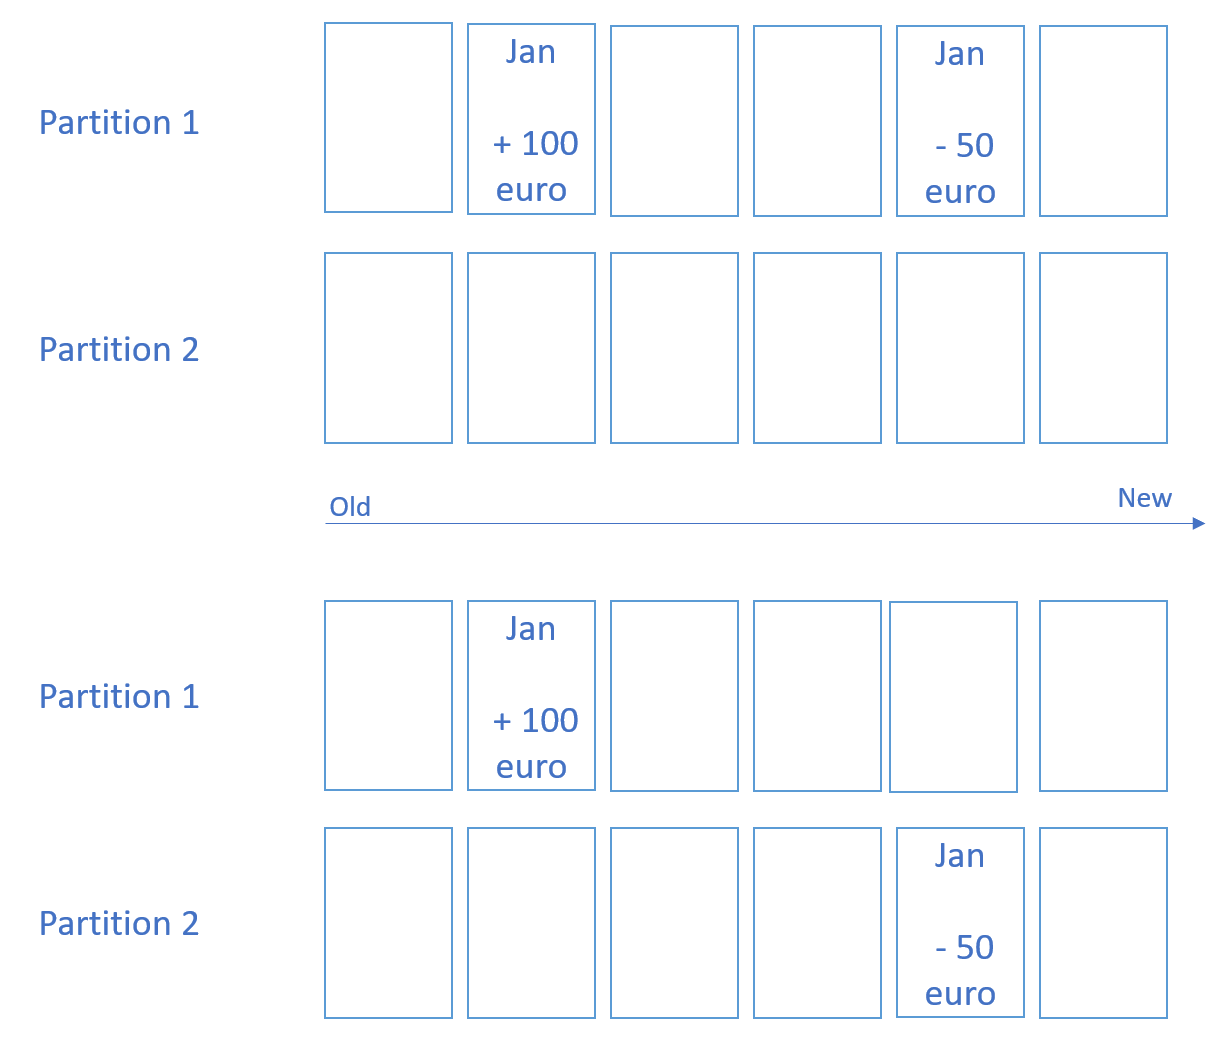
\includegraphics[scale=0.5]{partitions-example.png}
    \caption{De verdeling van ons voorbeeld over 1 partitie (met sleutel) of 2 partities (zonder).}
\end{figure}

Om vorig scenario te vermijden worden events aan partities toegewezen op basis van de sleutel van het event. Het is dus aan de producer om de juiste sleutel te kiezen, in dit geval ``Jan'', om ervoor te zorgen dat beide events op dezelfde partitie komen en allebei in de juiste volgorde aan de consumer worden bezorgd.
\newline
\newline


\section{Zookeeper}
ZooKeeper is een gedistribueerde service die het beheer van clusters en dus van grote hoeveelheden servers (nodes) helpt in goede banen te leiden. Dit op zich vormt een complexe taak en door die uit te besteden aan een oplossing zoals ZooKeeper kunnen andere gedistribueerde applicaties focussen op de eigen functionaliteiten en moeten ze geen ontwikkelingstijd stoppen in het oplossen van de typische problemen van parallelle systemen. Bijvoorbeeld ``deadlock'', waarbij 2 of meer processen op elkaar wachten en dus elkaar voor altijd blokkeren, en ``race conditions'' waarbij meerdere processen dezelde data terzelfdertijd willen verwerken. 
Zookeeper houdt ook centraal bepaalde data bij, zoals configuratie informatie, en maakt die beschikbaar voor alle nodes \autocite{ASF2023}.
\newline
\newline 
Bij Apache Kafka werd Zookeeper gebruikt voor metadata beheer, bijvoorbeeld bijhouden welke brokers allemaal deelmaken van de cluster. Daarnaast helpt Zookeeper bij het kiezen van een broker die de leider moet worden van een bepaalde partitie. In recente versies is dit vervangen door een intern systeem, wat als voordeel heeft dat gebruikers dan geen extra applicatie moeten leren opzetten en er worden ook minder resources gebruikt.
\autocite{Conduktor2023}
\newline
\newline
Afhankelijk van de versie van Kafka die we uiteindelijk zullen gebruiken kan Zookeeper wel of niet toegevoegd worden aan de oplossing.
\newline
\newline

\section{Big Data software Docker images}
Enkele van de Docker images die tijdens de cursus gebruikt worden zijn die van Big Data Europe. Dit is een project van de Europse Unie dat liep van 2015 tot 2017.
Eén van de doelstellingen was ``Design, integrate and deploy a cloud-deployment-ready Big Data aggregator platform comprising key open-source Big Data technologies for real-time and batch processing, such as Hadoop, Cassandra and Storm.'' \textcite{Commission2022}, dus om het voor Europese instellingen en bedrijven eenvoudiger te maken om in te stappen in het gebruik van deze Big Data oplossingen.
\newline
\sloppypar Op dockerhub zijn de images terug te vinden onder de bde2020 gebruiker (https://hub.docker.com/u/bde2020). Op github (https://github.com/big-data-europe) zijn alle sources te vinden van ieder image.
\newline
De laatste images van Spark en Hadoop zijn van vorig jaar (3.3.0) en er zijn geen images beschikbaar voor de laatste versie van Spark (3.4.0). Het is niet duidelijk of dit project nog zeer actief is. In de toekomst zullen we de images dus mogelijks zelf moeten bouwen, waarbij wel een beroep kan gedaan worden op de bestaande sources, of kijken naar andere publishers.
\newline
\sloppypar Bitnami is een ``Verified Publisher'' op Dockerhub, die dus te vertrouwen is, die een onder andere een Spark image ter beschikking stelt en Apache (https://hub.docker.com/u/apache) is een gesponsorde publisher die o.a. Hadoop en Spark images aanbiedt.


\section{Virtual IT Company (VIC)}
VIC is een ``bedrijf'' van HOGENT dat virtuele machines voorziet voor studenten, zodat bepaalde oplossingen niet op een eigen computer moeten draaien. Op aanvraag van studenten worden virtuele machine(s) opgezet en wordt er een soort van contract afgesproken met machine specs en lifespan.
\newline
\newline
De infrastructuur van VIC HOGENT is gebaseerd op virtuele machines op de eigen hardware die wordt beheerd door VMware vSphere (VMware's virtualization platform) versie 8, waarvan de 2 belangrijkste onderdelen ESXi en vCenter Server zijn.
\newline
VMWare ESXi is de naam van de VMWare hypervisor en is dus het virtualisatie platform waarop virtuele machines worden uitgevoerd en vCenter Server is de service waarmee alles beheerd wordt.
\newline
vCenter Server is een tool van VMware die toelaat toe om centraal het beheer te doen van de ESXi hosts, de virtuele machines, de netwerkinfrastructuur, de opslag en de gerelateerde componenten.
\newline
Volgens \textcite{VMware2023a} is een hypervisor software die op een fysieke machine draait en toelaat om op die machine meerdere virtual machines (VMs) te starten. Daartoe worden bepaalde resources van de fysieke machine, zoals geheugen, CPU en disk, gedeeld met alle virtuele machines.
\newline
Volgens \textcite{VMware2023b} is de vSphere oplossing leider in traditionele virtualisatie, gebaseerd op Virtuele machines.
\newline
Applicatie virtualisatie, waarbij elke applicatie in een aparte container draait, wordt steeds belangrijker, en voor dit soort aanpak zijn Docker containers de standaard oplossing. Om hieraan tegemoet te komen werd door VMWare voor vSphere 6 'vSphere Integrated Containers' ontwikkeld, een oplossing die toelaat om Docker images en containers te gebruiken op bestaande vSphere infrastructuur. Toevallig heet dit ook VIC \autocite{VMware2023b}.
Deze oplossing ondersteunt ook het deployen van Multi-Container Applicaties, o.a. door het gebruik van Docker Compose files.
\newline
\newline
Volgens \textcite{VMware2021} is Kubernetes intussen de de-facto standaard geworden voor de orchestratie en het beheer van containers op grote schaal, dus zijn Docker containers en Kubernetes nu geïntegreerd vanaf vSphere versie 7. De 'vSphere Integrated Containers' oplossing van vSphere 6 wordt niet langer ondersteund en ook Docker Compose niet meer.
\newline
\newline
Kubernetes wordt door vSphere vooral ondersteund om ontwikkelaars te laten werken met de door hun gekende tools, begrippen, Kubernetes configuratie files en processen zodat ze zich niet moeten verdiepen in VMWare vSphere. Ze hebben dan ook geen directe toegang of kennis nodig van de vSphere software.\autocite{VMware2019}
\newline
\newline
Daarnaast worden ook Docker containers ondersteund door VMWare vSphere, dus dit is een mogelijke oplossing zonder Kubernetes.
\newline
\newline
Kubernetes wordt door vSphere ondersteund op 2 manieren: ofwel door gebruik te maken van de vSphere Pods waarbij het beheer van de Docker containers nog steeds via de traditionele vSphere Admin verloopt, die een subset van de Kubernetes configuratie ondersteunt, ofwel via de Tanzu Kubernetes cluster. Dit is software van VMWare die apart kan worden geïnstalleerd en die de Kubernetes manier van werken ondersteunt en dus ook meer controle biedt over het beheer van de Kubernetes cluster.
\newline
\newline
Momenteel wordt er nog geen Kubernetes gebruikt in het VIC en is Tanzu Kubernetes ook niet geïnstalleerd. Het integreren van Kubernetes is een omvangrijke taak waar op dit moment binnenin het VIC geen resources voor zijn (dit zou een bachelorproef op zichzelf zijn).
\newline
Containertechnologie zoals Docker containers en Docker Compose wordt al meer dan een jaar gebruikt, waarbij de Docker Engine geïnstalleerd is in virtuele machines.
\newline
\newline
De volgende componenten zijn van belang om het gebruik van Kubernetes op VMware te begrijpen. De concepten van Kubernetes worden gelinkt aan VMWare concepten.
\newline
\newline
\subsection{Nodes}
Een Kubernetes node kan een virtuele of fysieke machine zijn die deel uitmaakt van een Kubernetes cluster en die centraal beheerd wordt.
Er zijn 2 types nodes:
\begin{itemize}
    \item ``master'' node: ook de ``control plane'' van Kubernetes genoemd. Deze controleert de volledige cluster en een cluster moet minstens 1 master node bevatten, en voor robuustheid typisch 2.
    \item ``worker'' node: bevat de nodige services om Pods (zie verder) te kunnen starten, deze bevatten de containers.
\end{itemize}
\autocite{NirShtein2023}
%\newline
%\newline
\subsection{Pod}
Een Kubernetes Pod is een groep van 1 of meerdere containers die samen draaien in een gedeelde context. Een pod wordt beheerd door de Kubelet software die op elke Node draait, de Kubelet zorgt ervoor dat Pods herstart worden als ze onverwachts stoppen of als hun configuratie is gewijzigd. Die configuratie is gelijkaardig aan een Docker Compose file en bevat één of meerdere container definities, de poorten die opengesteld moeten worden, de opslagvolumes, environment variabelen, enz 
\autocite{NirShtein2023}.

Een master node komt overeen met vCenter Server en een worker node is een machine waarop de ESXi hypervisor draait, en die dus kan Pods starten. Vanuit VMware Administrator standpunt is een Pod gelijkaardig aan een virtuele machine \autocite{VMware2019}.


\subsection{Namespace}
Namespaces zijn een mechanisme om de beschikbare resources binnen een Kubernetes cluster in te delen in groepen en dan die groepen toe te wijzen aan teams van gebruikers of projecten. Dit is vooral nuttig indien meerdere personen rechtstreeks gebruik maken van Kubernetes om zelf containers te deployen. Dit is hier niet aan de orde, het is de bedoeling dat alle installaties uitgevoerd worden door een administrator, dus Kubernetes Namespaces zijn hier van geen belang. Volgens \textcite{Kubernetes2023c} zijn Namespaces ook niet bedoeld voor kleine clusters tot enkele tientallen gebruikers. Namespaces zijn vergelijkbaar met vSphere Resource Pools volgens \textcite{VMware2019}.
